
\chapter{Choix technologique}
\label{chap:choix}

\section{Rappel de notre projet}

Suite à notre état de l'art, nous avons décidé de réaliser notre système de détection en installant un maillage de capteur qui se baseront sur le système du Montréal 3V2. Chaque capteur sera connecté à un \rpi 2 \footnote{La documentation technique du Raspberry PI est situé en annexe à la page \pageref{annexe:rpi}}. De plus, chaque \rpi communiquera avec un ordinateur central qui traitera les données pour les afficher sur une interface graphique. Les données qui seront transmises sont: le numéro du \rpi, la position du capteur, et le gisement du drone par rapport au capteur. Enfin, l'ordinateur central communiquera avec une application android qui notifiera le client de la présence d'un drone.
~\\

L'architecture physique du système est présenté à la figure \ref{fig:arch_phys}.

\begin{figure}[!h]
  \centering
  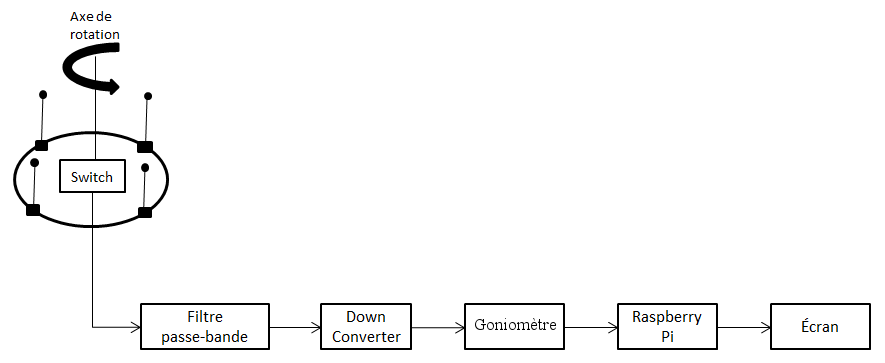
\includegraphics[width=\textwidth]{fonctionnement}
  \caption{Architecture Physique}
  \label{fig:arch_phys}
\end{figure}


\begin{figure}[!h]
  \centering
  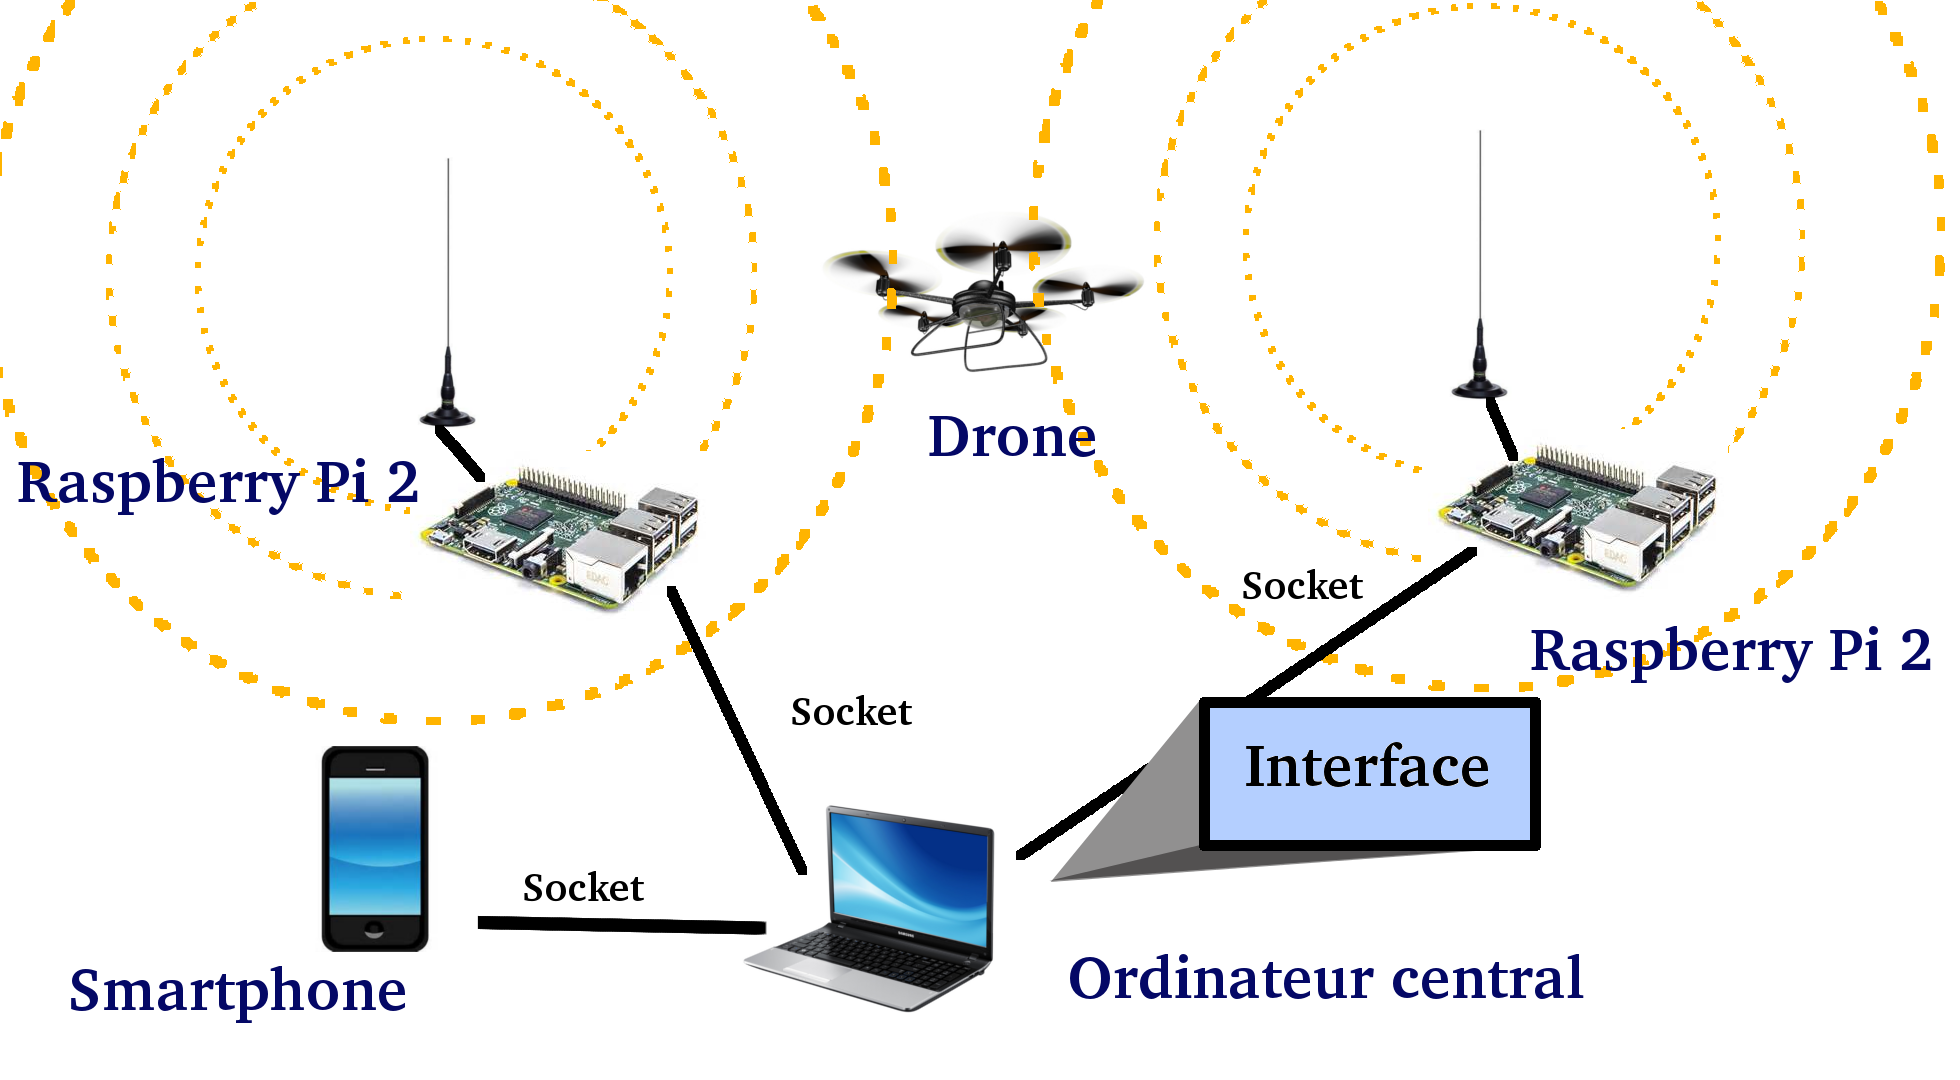
\includegraphics[width=\textwidth]{installation}
  \caption{Installation de Smart}
  \label{fig:inst}
\end{figure}



%%% Local Variables: 
%%% mode: latex
%%% TeX-master: "../rapport"
%%% End: 
